% This must be in the first 5 lines to tell arXiv to use pdfLaTeX, which is strongly recommended.
\pdfoutput=1
% In particular, the hyperref package requires pdfLaTeX in order to break URLs across lines.

\documentclass[11pt]{article}

% Change "review" to "final" to generate the final (sometimes called camera-ready) version.
% Change to "preprint" to generate a non-anonymous version with page numbers.
\usepackage[preprint]{acl}

% Standard package includes
\usepackage{times}
\usepackage{latexsym}

% For proper rendering and hyphenation of words containing Latin characters (including in bib files)
\usepackage[T1]{fontenc}
% For Vietnamese characters
% \usepackage[T5]{fontenc}
% See https://www.latex-project.org/help/documentation/encguide.pdf for other character sets

% This assumes your files are encoded as UTF8
\usepackage[utf8]{inputenc}

% This is not strictly necessary, and may be commented out,
% but it will improve the layout of the manuscript,
% and will typically save some space.
\usepackage{microtype}

% This is also not strictly necessary, and may be commented out.
% However, it will improve the aesthetics of text in
% the typewriter font.
\usepackage{inconsolata}

%Including images in your LaTeX document requires adding
%additional package(s)
\usepackage{booktabs}
\usepackage{graphicx}
\usepackage{hyperref}

\graphicspath{{images/}}

\title{Classifying Movie Reviews into the Six Ekman Emotions}

\author{Victor Verma \\
Boston University \\
\texttt{vpverm@bu.edu}}

\begin{document}
\maketitle
\begin{abstract}
\end{abstract}

\section{Introduction}
I plan to determine the most prevalent emotions expressed in user movie reviews for 65 of the top 250 highest rated movies on Letterboxd. Specifically, I will consider Ekman's six basic emotions: happiness, sadness, anger, fear, disgust, and surprise \textbf{[CITATION NEEDED HERE]}. To collect the source data, I will write a python script that scrapes the reviews (several thousand for each movie) from Letterboxd. In total, I expect to aggregate about 78,000 total reviews for analysis, and I can extend to a larger set of movies if more reviews are needed. \\ \\
Although excellent text-to-emotion models already exist, I will make my own from scratch. This will be created by training a model using supervised learning on a large text dataset labeled with the six basic emotions. I aim to experiment with logistic regression, support vector machines, random forests, and neural networks, and use the model that performs the best. After identifying the most effective text-to-emotion classification model, I intend to apply it to the unlabeled dataset of movie reviews. As someone who loves movies, I am curious to learn if there is a common set of emotions that audiences express after watching highly rated movies. \\ \\
There will be two parts to my final report. The first section will focus on evaluating the effectiveness of the emotion classification models that I will have created based on the standard metrics of accuracy, precision, recall, and F1 score. Here I will also try to account for any significant differences in model performance and any potential limitations. The second section will interpret the results of the emotional classification of the Letterboxd movie reviews. This will include summarizing simple statistics, such as the frequencies of each emotion, as well as identifying less obvious patterns that might emerge when grouping emotions together or stratifying by movie metadata (e.g. release year). For example, I am interested to see if there are traditionally unrelated genres that generate similar emotional reactions. \\ \\
Although the text-to-emotion classification methods are not novel, their applications to Letterboxd movie reviews will draw significant interest. I actively maintain a \href{https://www.recommendations.victorverma.com/}{movie recommendation website} that generates recommendations using machine learning based on a user's Letterboxd profile, and has accumulated nearly 1,800 users to date. I intend to present my findings on the website since there is so much topical overlap, and the results may enable users to better understand their own movie-watching identity.

\section{Data}
\subsection{Letterboxd Movie Reviews}
The unlabeled movie review data was sourced from Letterboxd's \href{https://letterboxd.com/dave/list/official-top-250-narrative-feature-films/}{Official Top 250 Narrative Feature Films}. Although the list contains 250 movies, data was only used from the 65 that I had previously seen. The official list is updated weekly, but the collected data is from February 24th, 2024. \\ \\
For each movie, the first 1,200 reviews sorted in order of decreasing activity were scraped. Each individual review was organized as a JSON object containing the author's rating of the movie, the date of the review, the number of comments left on the review, the review text itself, and the number of likes the review received. These were aggregated in a CSV with the JSON fields as columns. \\ \\
Several steps were taken to preprocess the movie review data. First, all of the None and NaN reviews were dropped. Next, the emojis were converted into their text equivalent, enclosed by a colon on each side. Non-English language reviews were then removed for convenience, as well of those solely consisting of punctuation. Finally, unnecessary whitespaces and newline characters were deleted to minimize the length of each review. \\ \\
The processed dataset contained 65,803 movie reviews, with each receiving 153 likes and 3 comments on average. The distribution of ratings given by the user to the movie being reviewed, measured on scale of 0.5 - 5.0, is summarized in \hyperref[tab:review_rating_distribution]{Table 2.1.1}. From the counts, it can be seen that most of the ratings associated with reviews were high, which was expected given that the source movie data is a list of highly rated movies. This led to the baseline expectation that positive emotions would likely be expressed most often in the dataset.
\renewcommand{\thetable}{2.1.1}
\begin{table}[h]
    	\centering
    	\begin{tabular}{c c c}
        		\toprule
        		\textbf{Rating} & \textbf{Number of Reviews} & \textbf{Percentage} \\
        		\midrule
        		None & 1,858 & 2.82\% \\
        		0.5 & 400 & 0.61\% \\
        		1.0 & 237 & 0.36\% \\
        		1.5 & 132 & 0.20\% \\
        		2.0 & 366 & 0.56\% \\
        		2.5 & 471 & 0.72\% \\
        		3.0 & 1,209 & 1.83\% \\
        		3.5 & 2,329 & 3.54\% \\
        		4.0 & 8,586 & 13.05\% \\
        		4.5 & 13,589 & 20.65\% \\
        		5.0 & 36,321 & 55.20\% \\
        		\bottomrule
    	\end{tabular}
    	\caption{Distribution of Movie Ratings}
    	\label{tab:review_rating_distribution}
\end{table}
\subsection{Twitter Emotion Corpus}
The labeled emotion data was sourced from the \href{https://socialmediaie.github.io/MetaCorpus/#:~:text=Hashtag\%20Emotion\%20Corpus\%20(aka\%20Twitter\%20Emotion\%20Corpus,\%20or\%20TEC)}{Twitter Emotion Corpus (TEC)}. The raw .txt file was parsed into a CSV with the text and emotion label as columns, and preprocessed in a similar manner as the movie review data. First, the emojis were converted into their text equivalent, enclosed by a colon on each side. Next, non-English language reviews were removed for convenience, as well of those solely consisting of punctuation. Finally, unnecessary whitespaces and newline characters were deleted to minimize the length of each review. \\ \\
The processed dataset consisted of 19,333 text-label pairs, and the distribution of labels is shown in \hyperref[tab:emotion_label_distribution]{Table 2.2.1}. It would have been ideal to have an approximately equal share of samples for each emotion label, but no such dataset was found.
\renewcommand{\thetable}{2.2.1}
\begin{table}[h]
    	\centering
    	\begin{tabular}{c c c}
        		\toprule
        		\textbf{Emotion} & \textbf{Count} & \textbf{Percentage} \\
        		\midrule
        		Happiness & 7,892 & 40.82\% \\
        		Sadness & 3,613 & 18.69\% \\
        		Anger & 1,489 & 7.70\% \\
        		Fear & 2,563 & 13.28\% \\
        		Disgust & 733 & 3.79\% \\
        		Surprise & 3,043 & 15.74\% \\
        		\bottomrule
    	\end{tabular}
    	\caption{Distribution of Emotion Labels}
	\label{tab:emotion_label_distribution}
\end{table}

\section{Baseline}
As a starting point, an \href{https://huggingface.co/arpanghoshal/EkmanClassifier}{Ekman Classifier (EC)} model from HuggingFace was used for emotion inference. It was built using the BertForMultiLabelClassification model architecture and finetuned using Google's \href{https://huggingface.co/datasets/google-research-datasets/go_emotions}{GoEmotions} dataset. The model supported labeling the standard Ekman emotions, plus "neutral". \\ \\
To get an initial baseline, the EC model was evaluated upon the processed TEC dataset. Labels predicted as "neutral" were discarded because the label is not present in the TEC dataset. Surprisingly, the model only had an accuracy rate of 43.94\%, much lower than expected from a pre-trained model. \\ \\
The precision, recall, and F1-score are summarized in \hyperref[tab:baseline_summary_statistics]{Table 3.1}. Only two out of six emotions, fear and sadness, had a precision score greater than 0.5. This suggested that the baseline model produced a large number of false positives. Only one emotion, happiness, had a recall score greater 0.5, suggesting that the baseline model produced a large number of false negatives too. Consequently, only happiness had an F1-score greater than 0.5, indicating that the baseline model was objectively not very good at classifying the Ekman emotions. \\ \\
\renewcommand{\thetable}{3.1}
\begin{table}[h]
    	\centering
    	\begin{tabular}{c c c c}
        		\toprule
        		\textbf{Emotion} & \textbf{Precision} & \textbf{Recall} & \textbf{F1-Score} \\
        		\midrule
        		Happiness & 0.47 & 0.74 & 0.58 \\
        		Sadness & 0.56 & 0.31 & 0.40 \\
        		Anger & 0.28 & 0.42 & 0.34 \\
        		Fear & 0.76 & 0.21 & 0.33 \\
        		Disgust & 0.26 & 0.09 & 0.14 \\
        		Surprise & 0.26 & 0.22 & 0.24 \\
        		\bottomrule
    	\end{tabular}
    	\caption{EC Model Summary Statistics}
	\label{tab:baseline_summary_statistics}
\end{table}
The failures of the EC model were further investigated using the confusion matrix displayed in \hyperref[fig:baseline_confusion_matrix]{Figure 3.2}, which allowed for insight into how emotions were being mislabeled. For example, it was seen that happiness was commonly mistook for surprise, which potentially makes sense because there can sometimes be overlap between the two emotions. On the other hand, happiness and sadness were sometimes confused for each other, which was not expected since they are semantically opposite. Interestingly, the model had a hard time identifying anger and fear, with somewhat uniform mislabel distributions, which was surprising because one might consider these emotions to read as relatively distinct in text. The EC model served as a good starting point, but it did not work as well as expected.
\renewcommand{\thefigure}{3.2}
\begin{figure}[h]
	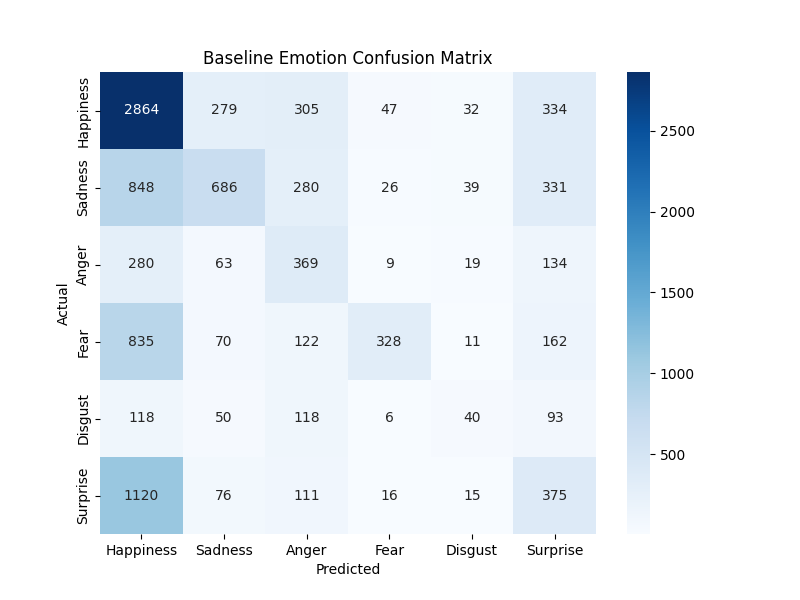
\includegraphics[width=0.5\textwidth]{baseline_emotion_confusion_matrix.png}
	\caption{EC Model Confusion Matrix}
	\label{fig:baseline_confusion_matrix}
\end{figure}
\section{Models}

\section{Application}

\section{Limitations}

\section{Acknowledgements}

\section{References}

\end{document}
